\documentclass{beamer}
\usepackage{graphicx}
\usepackage[english]{babel}
\usepackage{etoolbox}
\usepackage[autostyle, english=american]{csquotes}
\MakeOuterQuote{"}

\graphicspath{{images/}{plots/}}

\title{Effect of Jupiter-sized Planet Interactions on Planetary Systems}
\author{Tyler Reisinger}
\date{}

\begin{document}

\begin{frame}{Background}
    \begin{columns}
        \column{0.66\textwidth}
        \begin{itemize}
            \item Explore formation scenarios for Hot Jupiters (HJs) in planetary
                systems.
                \begin{itemize}
                    \item Jupiter-mass planets orbiting very close to their host star.
                    \item An estimated 1\% of planetary systems contain a 
                        Hot Jupiter (A. Brucalassi et al. 2016)\footnotemark.
                \end{itemize}
            \item Understand the side-effects of HJ formation.
                \begin{itemize}
                    \item Does the migration of the HJ affect other planetary orbits?
                    \item Are terrestrial planets in highly eccentric orbit a possible
                        indicator of Hot Jupiter formation.  
                \end{itemize}
        \end{itemize} 
        \column{0.34\textwidth}
            \begin{figure}
                \centering
                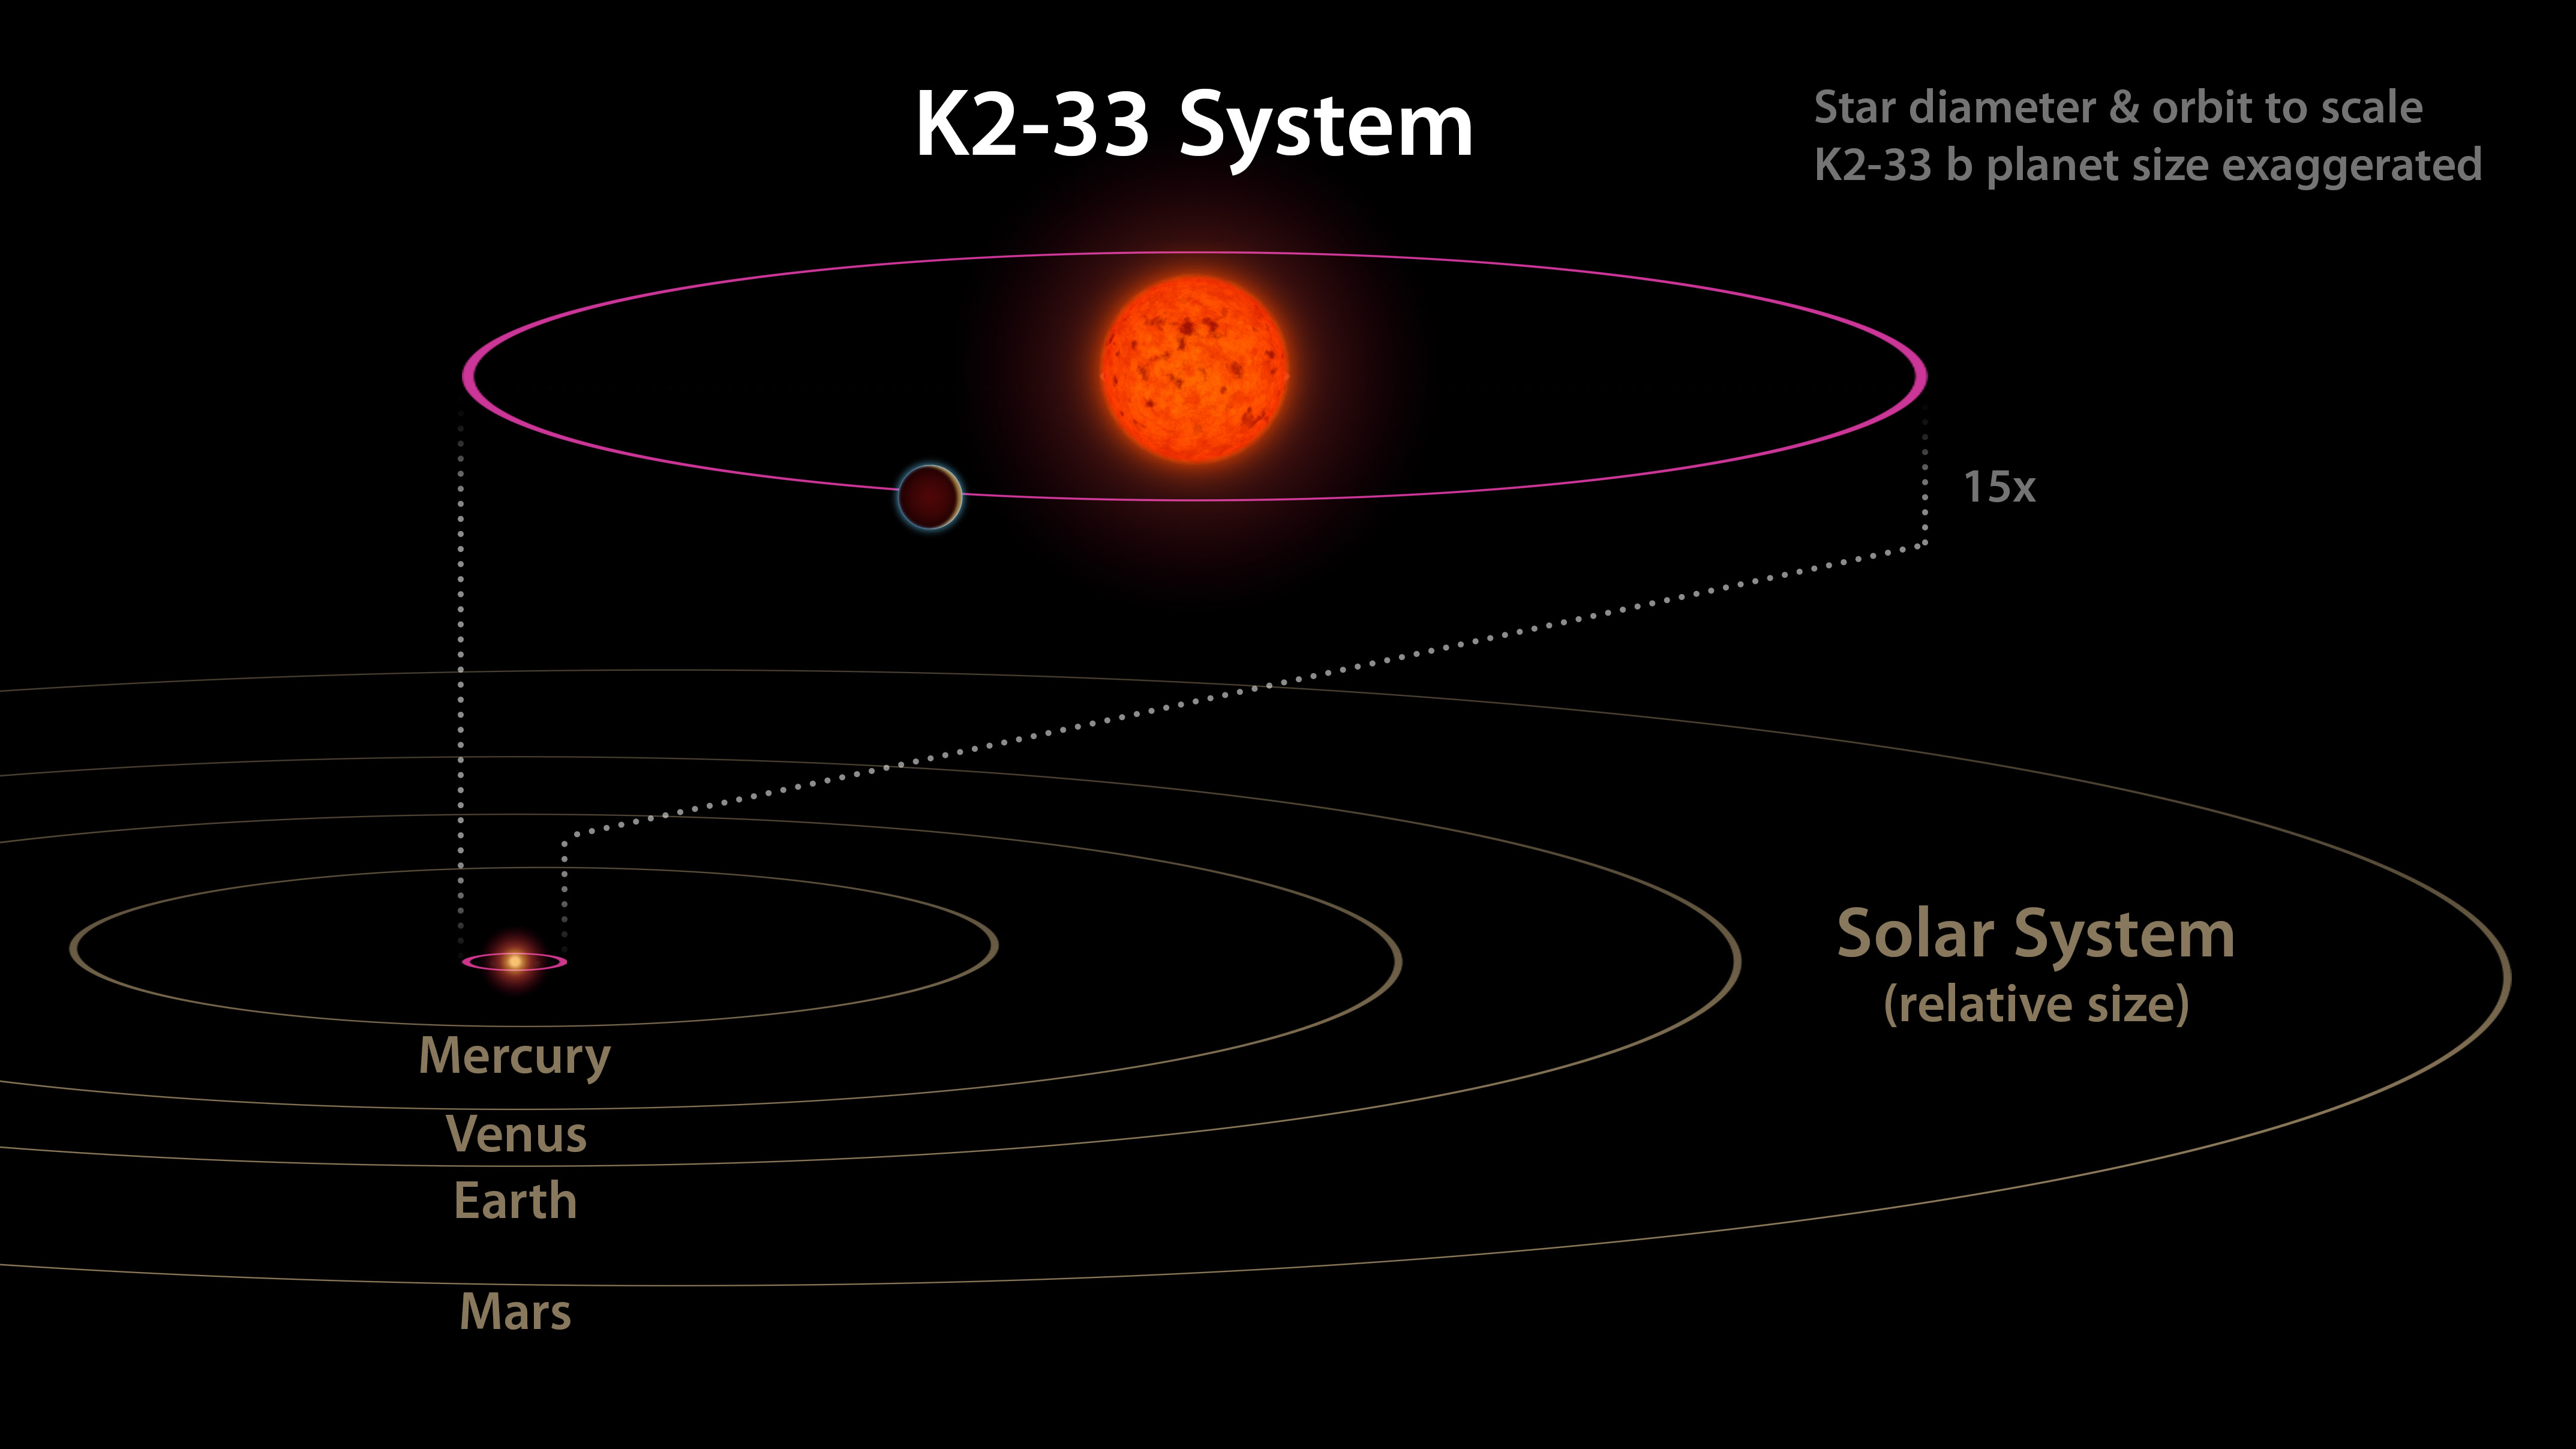
\includegraphics[width=1.66in]{hj_orbit}
            \end{figure}
    \end{columns}
    \footnotetext[1]{James B. Pollack, Olenka Hubickyj, Peter Bodenheimer, Jack J. Lissauer, Morris Podolak, Yuval Greenzweig, Formation of the Giant Planets by Concurrent Accretion of Solids and Gas, Icarus, Volume 124, Issue 1, 1996, Pages 62-85, ISSN 0019-1035, http://dx.doi.org/10.1006/icar.1996.0190.
(http://www.sciencedirect.com/science/article/pii/S0019103596901906) }

\end{frame}
\begin{frame}{Theory}
    \begin{columns}
        \column{0.67\textwidth}
        \begin{itemize}
            \item Scattering Effects
                \begin{itemize}
                    \item HJs starts like a normal gas planet, but is perturbed inward.
                    \item Perturbation may come from stellar interactions
                        within a star cluster.
                        \begin{itemize}
                            \item The star cluster may later dissolve, but the
                                damaging effects of an interaction would still be present.
                        \end{itemize}
                    \item This could cause other planets in the system to be
                        knocked into eccentric orbits by the HJ.
                        \begin{itemize}
                            \item Such an event might leave an observable impact on the 
                                planetary system.
                            \item If we understand what this might look like,
                                we can look for it in the universe.
                        \end{itemize}
                \end{itemize}
            \item We will use computational simulations to explore this scenario.
        \end{itemize}
        \column{0.33\textwidth}
            \begin{figure}
                \centering
                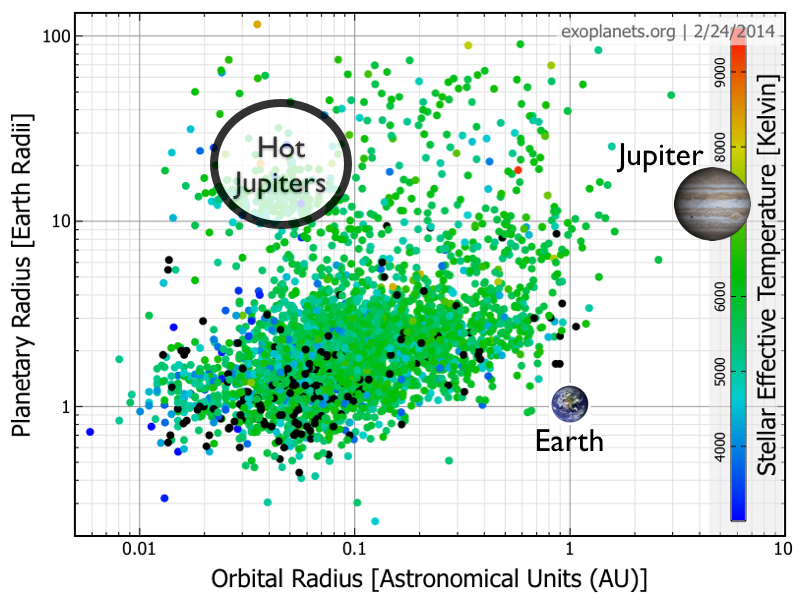
\includegraphics[height=1.25in]{hot_jupiter_measure_plot}
                %\caption{Artistic interpretation of an HJ around a star. Image: Haven Giguere, Nikku Madhusudhan}
            \end{figure}
    \end{columns}
\end{frame}
\begin{frame}{Cluster N-Body}
    \begin{itemize}
        \item King Model with $W_0 = 3.0$.
        \item Clusters of a few thousand stars are created and simulated.
        \item Each star has fixed $M = 1 M_{sun}$.
        \item Let AMUSE run the simulation, call back into user code for close
            stellar encounters.
        \item Compute and record:
            \begin{itemize}
                \item Dynamical parameters of each star.
                \item Orbital parameters $(a, e, r)$
                \item Distance of closest encounter
            \end{itemize}
        \begin{figure}
            \centering
            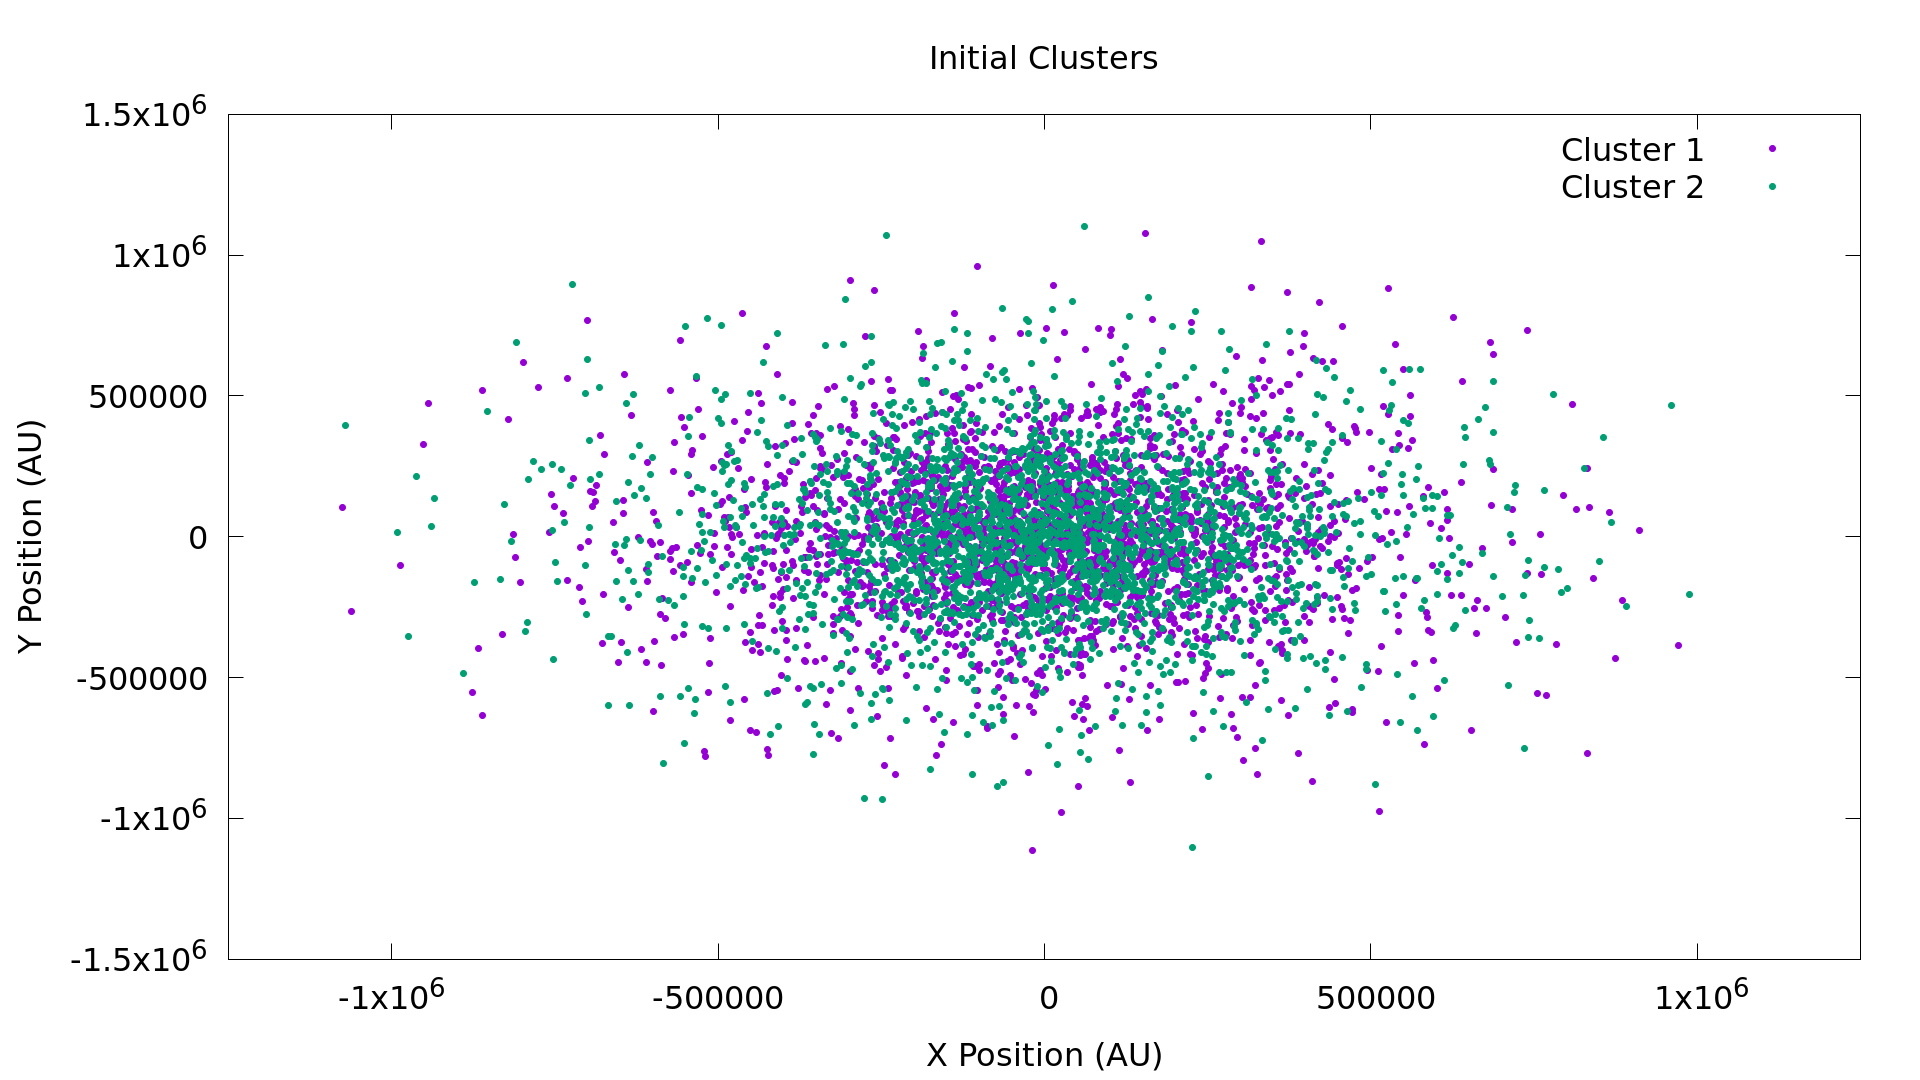
\includegraphics[height=1.5in]{cluster_superimposed.png}
        \end{figure}
    \end{itemize}

\end{frame}

\begin{frame}{Encounter Results}
    \begin{itemize}
        \item For a simulation of 4000 stars run for 150 Myr:
            \begin{itemize}
                \item There were 632 total encounters returned to us by AMUSE.
                \item Radius of closest encounter ranges between 0 and 300 AU.
                \item Only 7.5 \% of encounters are close enough to be
                    considered for planetary encounters ($<$ 30 AU).
            \end{itemize}
    \end{itemize}
    \begin{figure}
        \center
        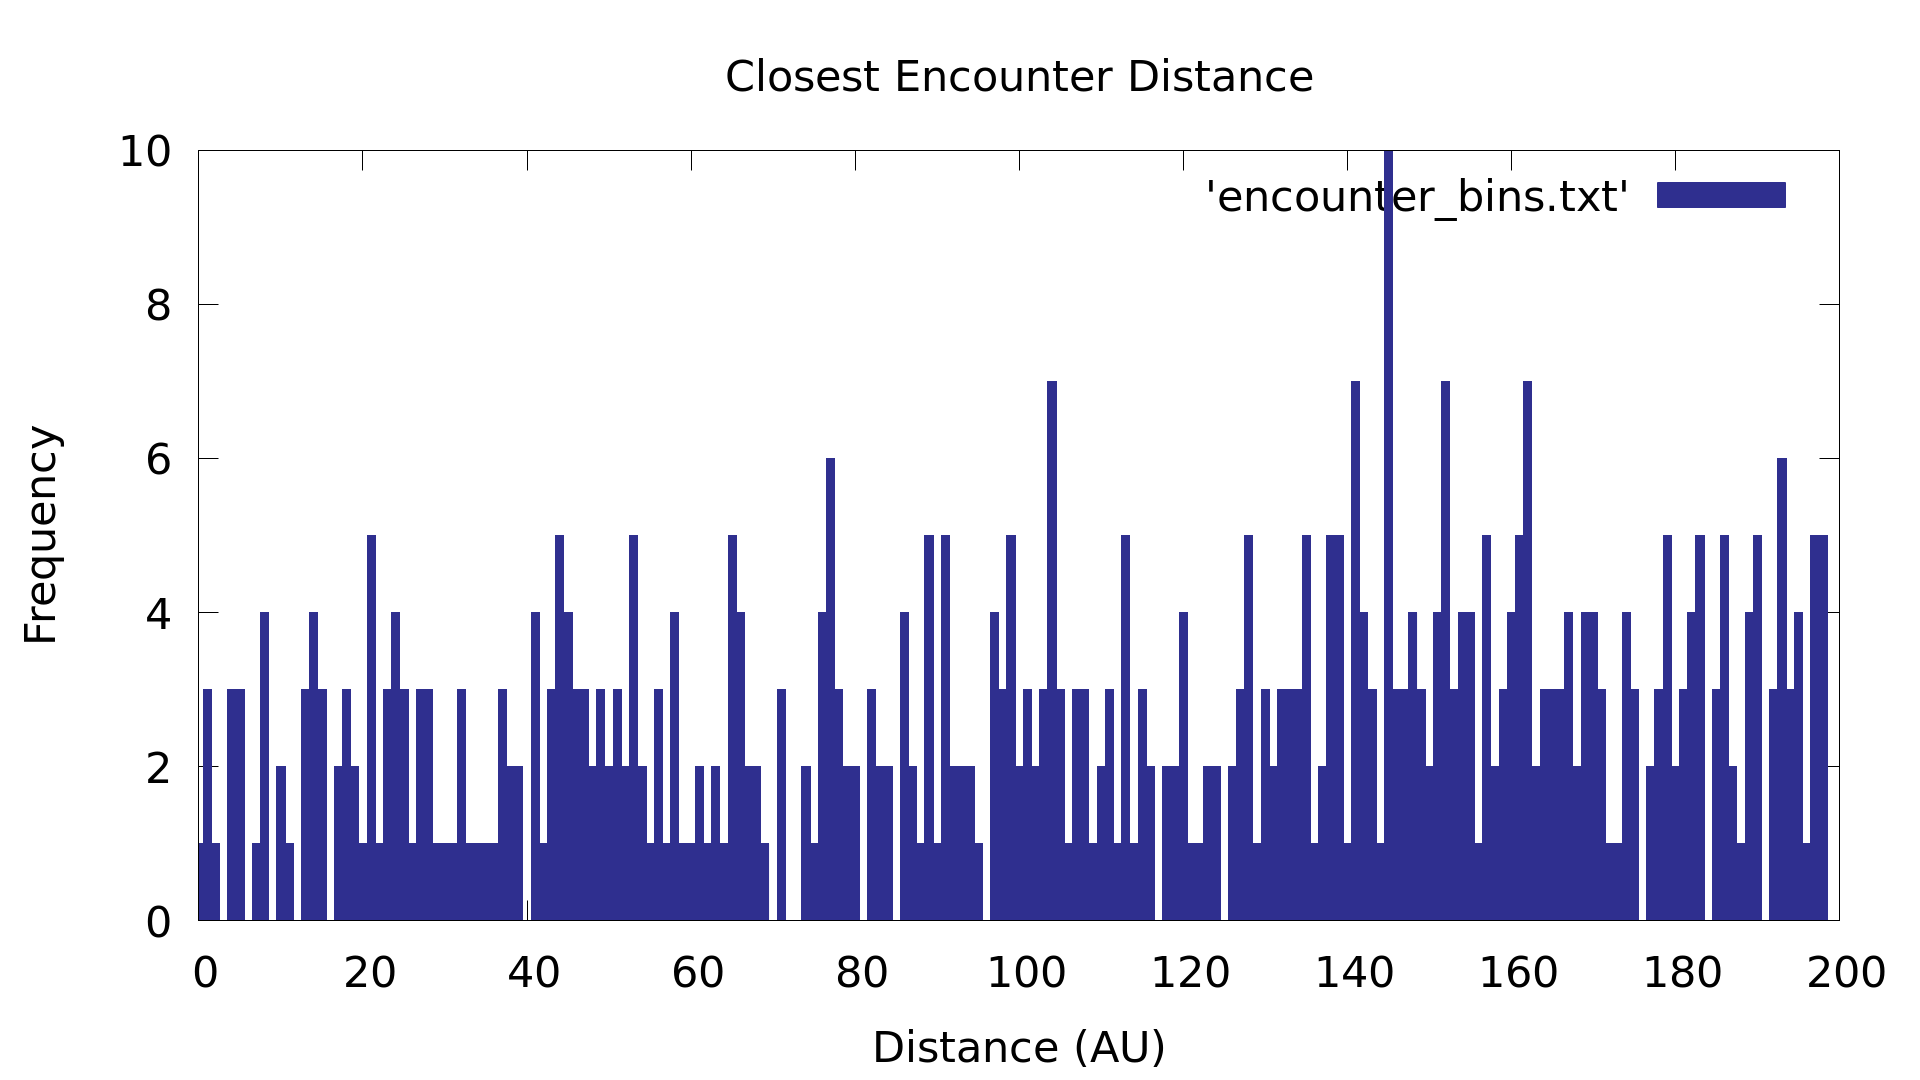
\includegraphics[width=2.5in]{encounter_dist}
    \end{figure}
\end{frame}

\begin{frame}{Stage 2: Monte-Carlo Simulations}
    \begin{itemize}
        \item Take the cluster encounter data and run detailed simulations.
        \begin{itemize}
            \item Initialize stars from encounter parameters.
            \item Ignore distant encounters.
            \item Add some planets, currently an Earth and Jupiter.
            \item Let run from recorded encounter.
            \item Store trajectories of all bodies.
            \item Simulate until encounter is "over".
        \end{itemize}
    \end{itemize}
    \begin{figure}
        \centering
        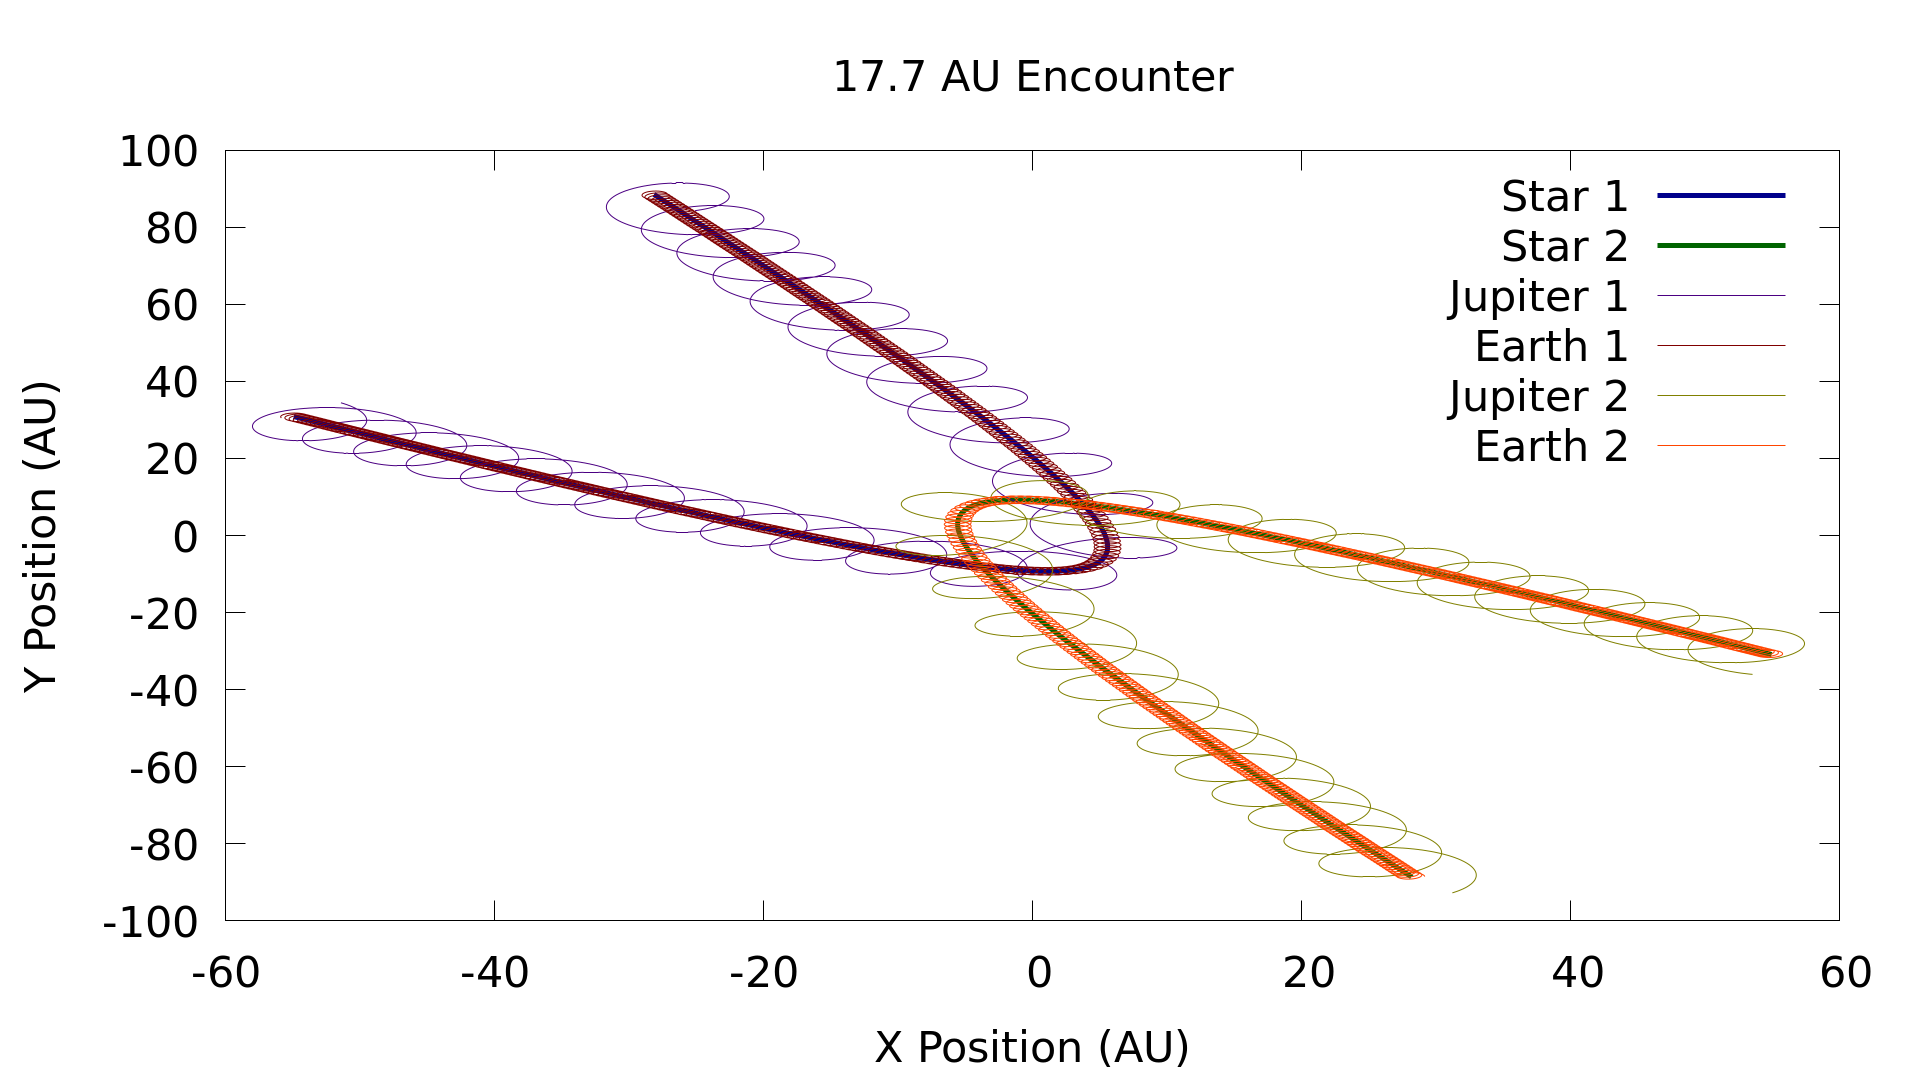
\includegraphics[height=1.75in]{17_7_AU}
    \end{figure}
\end{frame}

\end{document}
